\documentclass[8pt]{beamer}
\usepackage{tikz}
\usepackage[utf8]{vietnam}
\usepackage{amsmath}
\usepackage{graphicx}
\usepackage{mathrsfs}
\usepackage{amssymb,amsfonts,amsthm}
\usepackage{wrapfig}
\usepackage{hyperref}
\usetheme{Copenhagen}
\usecolortheme{spruce}
\setbeamertemplate{navigation symbols}{}
\setbeamertemplate{headline}{}
\setbeamertemplate{footline}{}
\title[Kết quả nghiên cứu tuần 2]
{Kết quả nghiên cứu tuần $2$}
\subtitle{Phòng thí nghiệm Thông tin Vô tuyến}
\author[Phòng thí nghiệm thông tin Vô tuyến]
{Tín Vũ}
\date[VLC 2021] % (optional)
{tinvu1309@gmail.com}
\begin{document}
\frame{\titlepage}
\begin{frame}{Mục lục}
\tableofcontents
\end{frame}
\begin{frame}{Tài liệu tham khảo}
\section{Tài liệu tham khảo}
Tài liệu tham khảo được sử dụng để nghiên cứu gồm: Antenna Theory (A.Balanis), Fundamentals of Physics (David Halliday, 10th version).
\\ Tài liệu bổ sung: \href{https://www.youtube.com/watch?v=bHIhgxav9LY}{The Big Misconception About Electricity}, \href{https://www.youtube.com/watch?v=EH2A8mZmM9M}{The Poynting Vector in a DC Circuit}
\end{frame}
\begin{frame}{Các tham số cơ bản của Antenna}
\section{Các tham số cơ bản của Antenna}
\begin{itemize}
	\item Beamwidth
\end{itemize}
\subsection{Beamwidth}
\begin{figure}[h]
			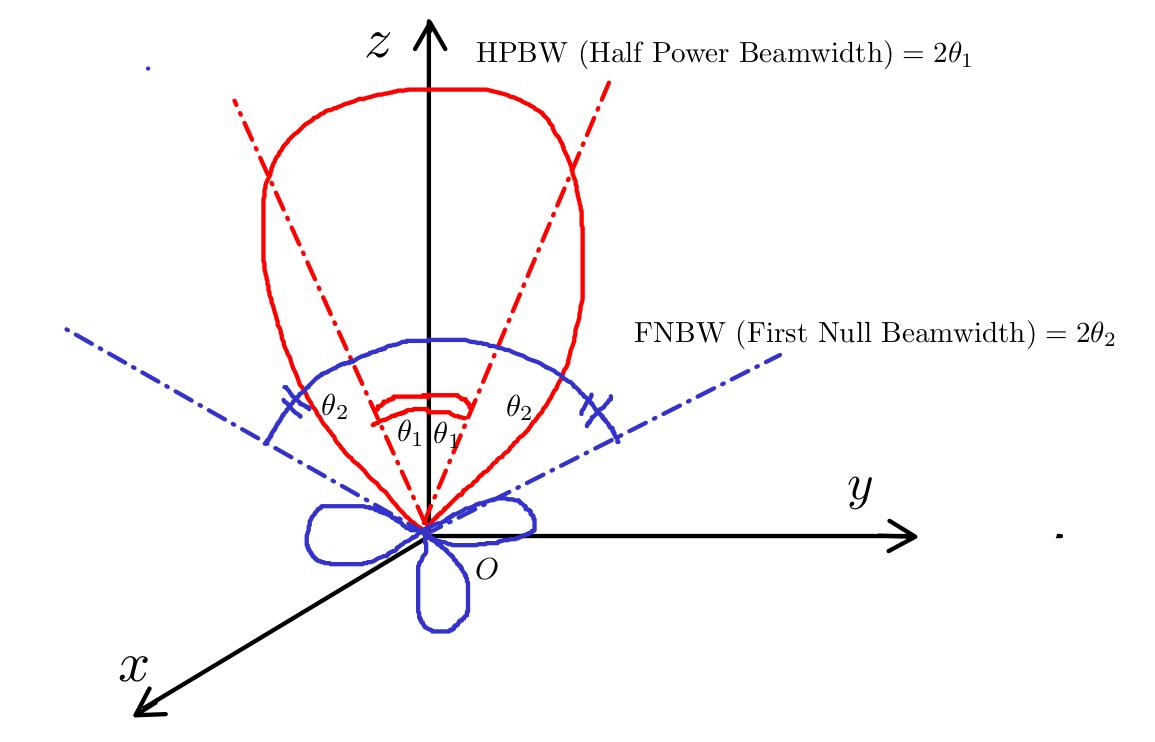
\includegraphics[width=0.9\textwidth]{beamwidth.jpg}
			\caption{Beamwidth model}			\label{fig:re1}
\end{figure}
\end{frame}
\begin{frame}{Các tham số cơ bản của Antenna}
 Theo IEEE, khái niệm "beamwidth" được định nghĩa là khoảng cách góc giữa hai điểm giống nhau đối xứng qua trục xác định.
\\ Trong quá trình thiết kế antenna, nếu giảm beamwidth thì side lobe tăng và ngược lại. 
\\ Ví dụ: antenna có cường độ bức xạ chuẩn hóa được biểu diễn như sau: 
$$U(\theta)=\cos^{2}{\theta}\cos^{2}{3\theta} \quad \left(0\leq\theta\leq\frac{\pi}{2},0\leq\phi\leq 2\pi\right)$$
Hãy tìm HPBW và FNBW.
\\ Từ công thức $U=r^2 W$ đã được thảo luận ở slide trước, ta thấy $U,W,P$ là 3 đại lượng tỉ lệ thuận với nhau. Hiển nhiên ta có:
$$P(\theta_{h})=\frac{1}{2}P(\theta)\Leftrightarrow U(\theta_{h})=\frac{1}{2}U(\theta)=\frac{1}{2}$$
Giải phương trình lượng giác trên, ta thu được giá trị $\theta_{h}=0.25\;(rad)$, vậy ta có $\text{HPBW}=2\theta_{h}=0.5\;(rad)$. Hoàn toàn tương tự, ta cũng dễ dàng tìm được FNBW:
$$U(\theta_{f})=0$$
Ta thu được 2 nghiệm $\theta_{f1}=\frac{\pi}{6}\;(rad)$ và $\theta_{f2}=\frac{\pi}{2}\;(rad)$. Nghiệm đầu tiên $\theta_{f1}$ chính là nghiệm của FNBW:
$$\text{FNBW}=2\theta_{f1}=\frac{\pi}{3}\;(rad)\quad (\text{side lobe angular})$$
Nghiệm thứ hai $\theta_{f2}$ chính là nghiệm của SNBW (second null beamwidth):
$$\text{SNBW}=2\theta_{f2}=\pi\;(rad)\quad (\text{back lobe angular})$$
Các kết quả này hoàn toàn khớp với mô hình đã được trình bày ở trên.
\end{frame}
\begin{frame}{Các tham số cơ bản của Antenna}
\begin{itemize}
	\item Directivity
\end{itemize}
\subsection{Directivity}
Khái niệm "directivity" của antenna được định nghĩa là tỉ số giữa cường độ bức xạ tại một hướng với cường độ bức xạ tại mọi hướng (của một antennna đẳng hướng đã được phân tích ở slide trước).
$$D(\phi,\theta)=\frac{U}{U_{0}}=\frac{U}{P_{rad}/(4\pi)}=\frac{4\pi U}{P_{rad}}$$
Trong hệ tọa độ cầu, chúng ta định nghĩa: $$D(\phi,\theta)=D_{\phi}+D_{\theta}$$
với: 
\begin{equation*}
\begin{split}
	D_{\phi}&=\frac{4\pi U_{\phi}}{(P_{rad})_{\phi}+(P_{rad})_{\theta}}\\
	D_{\theta}&=\frac{4\pi U_{\theta}}{(P_{rad})_{\phi}+(P_{rad})_{\theta}}
\end{split}
\end{equation*}
\end{frame}
\begin{frame}{Các tham số cơ bản của Antenna}
\subsubsection{Ví dụ 1}
Ví dụ 1: xét một antenna có độ chiếu xạ (irradiance):
$$W_{rad}=\hat a_{r}W_{r}=\hat a_{r}A_{0}\frac{\sin{\theta}}{r^2}\quad(W/m^2)$$
Với điều kiện bị giới hạn bởi mặt kín $S=\{(\phi,\theta)|0\leq\phi\leq2\pi,\;0\leq\theta\leq\pi\}$. Viết phương trình hàm $D(\phi,\theta)$ và tính $D_{max}(\phi,\theta)$.
Từ công thức: $$D(\phi,\theta)=\frac{U}{U_{0}}=\frac{4\pi U}{P_{rad}}$$
Ta cần xác định $U$ và $P_{rad}$:
$$P_{rad}=\iint_{S}W_{rad}\hat a_{r}da=\iint_{S}W_{rad}\hat a_{r}r^2\sin{\theta}d\theta d\phi=\int_{0}^{2\pi}\int_{0}^{\pi}A_{0}\sin^2{\theta}d\theta d\phi=\pi^2A_{0}$$
$$U=r^2W_{rad}=A_{0}\sin{\theta}\Rightarrow D(\phi,\theta)=\frac{4\sin{\theta}}{\pi}$$
Vậy ta có:
$$D(\phi,\theta)=\frac{4\sin{\theta}}{\pi}\Rightarrow D_{max}(\phi,\theta)=\frac{4}{\pi}$$

\end{frame}
\begin{frame}{Các tham số cơ bản của Antenna}
\subsubsection{Ví dụ 2}
Ví dụ 2: thực hiện tương tự yêu cầu như ví dụ 1, nhưng với độ chiếu xạ:

$$W_{rad}=\hat a_{r}W_{r}=\hat a_{r}A_{0}\frac{\sin^2{\theta}}{r^2}\quad(W/m^2)$$
Ta cần xác định $U$ và $P_{rad}$:
$$P_{rad}=\iint_{S}W_{rad}\hat a_{r}da=\iint_{S}W_{rad}\hat a_{r}r^2\sin{\theta}d\theta d\phi=\int_{0}^{2\pi}\int_{0}^{\pi}A_{0}\sin^3{\theta}d\theta d\phi=\frac{8\pi}{3}A_{0}$$
$$U=r^2W_{rad}=A_{0}\sin^2{\theta}\Rightarrow D(\phi,\theta)=\frac{3}{2}\sin^2{\theta}$$
Vậy ta có:
$$D(\phi,\theta)=\frac{3}{2}\sin^2{\theta}\Rightarrow D_{max}(\phi,\theta)=\frac{3}{2}$$
\end{frame}
\begin{frame}{Các tham số cơ bản của Antenna}
\subsubsection{Ví dụ 3}
Ví dụ 3: cho một antenna có phương trình hàm cường độ bức xạ của búp chính (main lobe) như sau:
$$U=B_{0}\cos^4{\theta}$$
Bức xạ này bị giới hạn bởi mặt kín $S=\{(\phi,\theta)|0\leq\phi\leq 2\pi\; ,0\leq\theta\leq\frac{\pi}{2}\}$. Tìm phương trình hàm $D(\phi,\theta)$, biết $B_{0}$ là hằng số.
\\ Ta có thể tiếp cận bài toán bằng hai hướng như sau:
\begin{equation*}
\begin{split}
	P_{rad}&=\iint_{S}Ud\Omega=B_{0}\iint_{S}\cos^4{\theta}\sin{\theta}d\theta d\phi=B_{0}\int_{0}^{2\pi}\int_{0}^{\frac{\pi}{2}}\cos^4{\theta}\sin{\theta}d\theta d\phi=\frac{B_{0}2\pi}{5}\\
	P_{rad}&=\iint_{S}Wda=\iint_{S}\frac{U}{r^2}r^2\sin{\theta}d\theta d\phi=\iint_{S}U\sin{\theta}d\theta d\phi=B_{0}\iint_{S}\cos^4{\theta}\sin{\theta}d\theta d\phi\\&=\frac{B_{0}2\pi}{5}
\end{split}
\end{equation*}
Vậy ta thu được:
$$D(\phi,\theta)=\frac{4\pi U}{P_{rad}}=10\cos^4{\theta}$$
Ta có: $D_{max}(\phi,\theta)=10$.
\\\alert{Thay vì biểu diễn các thông số không chiều (dimensionless), ta sẽ đổi chúng sang thang dB để tiện biểu diễn:}
$$D_{max}(dB)=10\log_{10}(D_{max}(\phi,\theta))$$
\end{frame}
\begin{frame}{Các tham số cơ bản của Antenna}
\subsubsection{Ví dụ 4}
Ví dụ 4: xác định hàm $D(\phi,\theta)$ của antenna sao cho $\text{HPBW}=\frac{\pi}{2}$, với:
$$U(\theta,\phi)=\sin^n{\theta}$$
Biết bức xạ lan tỏa trên toàn miền không gian.
\\ Ta thấy do $\text{HPBW}=\frac{\pi}{2}$, nên suy ra $\theta_{h}=\frac{1}{2}\frac{\pi}{2}=\frac{\pi}{4}$. Sử dụng kết quả của ví dụ 1, ta có:
$$U(\theta_{h},\phi)=\frac{1}{2}\Rightarrow \sin^n{\theta_{h}}=\frac{1}{2}\Rightarrow n=2$$
Do bức xạ lan tỏa trên toàn miền không gian, nên ta có $S=\{(\phi,\theta)|0\leq\phi\leq 2\pi\;, \ 0\leq\theta\leq\pi\}$.
\\ Vậy ta có:
$$P_{rad}=\iint_{S}Ud\Omega=\iint_{S}\sin^2{\theta}(\sin{\theta}d\theta d\phi)=\frac{8\pi}{3}$$
Và ta có thể dễ dàng suy ra:
$$D(\phi,\theta)=\frac{4\pi U}{P_{rad}}=\frac{3}{2}\sin^2{\theta}\Rightarrow D_{max}{(\phi,\theta)}=\frac{3}{2}$$
Đổi ra thang dB: $$D_{max}(dB)=10\log_{10}(D_{max}(\phi,\theta))=1.76dB$$
\end{frame}
\begin{frame}{Các tham số cơ bản của Antenna}
Đào sâu hơn một chút, thay vì chỉ dừng lại ở công thức, ta sẽ thử phác thảo radiation pattern của các antenna trong ví dụ 1 (2 giống 1, chỉ khác độ lớn), 3 và 4:

\begin{figure}[h]
			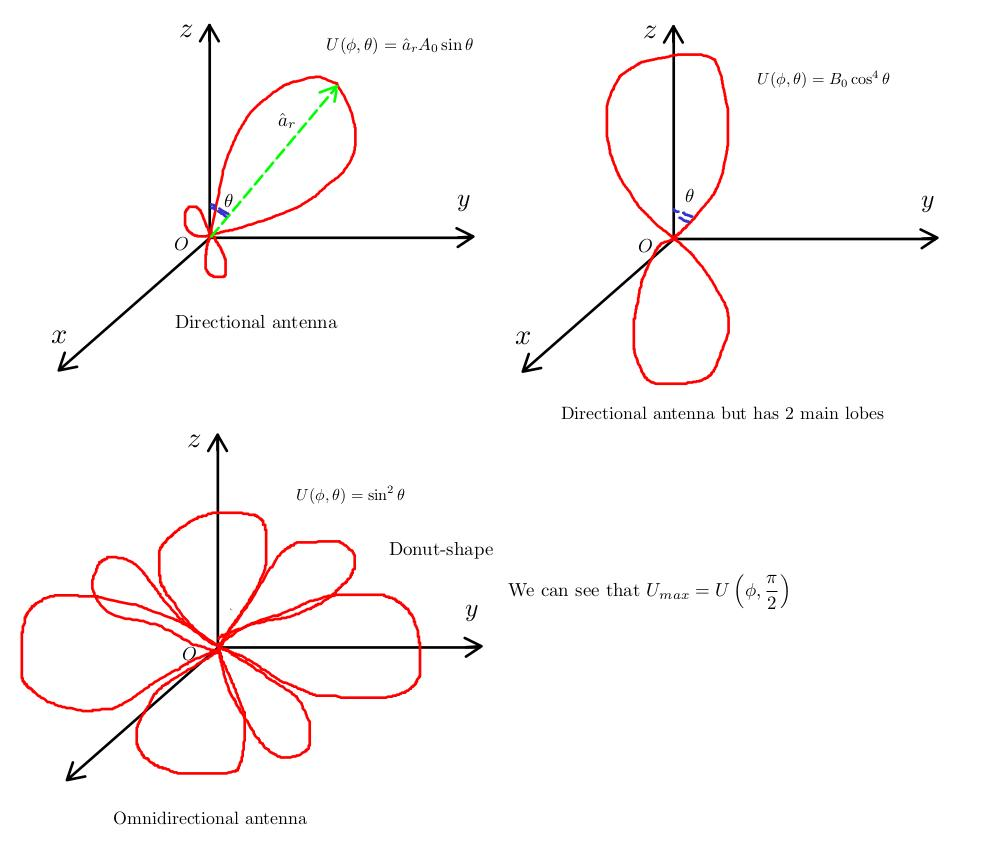
\includegraphics[width=0.75\textwidth]{omni.jpg}
			\caption{Directional and Omnidirectional antenna model}			\label{fig:re2}
\end{figure}
\end{frame}
\begin{frame}{Các tham số cơ bản của Antenna}
\subsection{Polarization}
\begin{itemize}
	\item Polarization
\end{itemize}
Trước khi đi sâu vào hiện tượng polarization (phân cực), ta sẽ nhắc lại các khái niệm cơ bản sau đã được thảo luận rất kĩ trong slide trước:
\begin{enumerate}
	\item Độ chiếu xạ của sóng EM: $$\mathscr{W}=\mathscr{E}\cdot\mathscr{H}=\frac{\mathscr{E}^2}{\mu_{0}c}$$
		Với hàm sóng $\mathscr{E}=E(x,y,z)e^{j\omega t}$, hay có thể biểu diễn dạng thực đơn giản hơn là $\Re{(\mathscr{E})}=E_{0}\sin(kx-\omega t)$, ta xây dựng công thức tính độ chiếu xạ trung bình như sau (một công thức tương tự đã được đề cập đến ở slide trước, nhưng sử dụng các hàm phức tương đối phức tạp với 4 biến):
		$$W=\frac{\int_{T}\mathscr{W}dt}{T}=\frac{\mathscr{E}^2}{2\mu_{0}c}=\frac{1}{\mu_{0}c}\left(\frac{\mathscr{E}}{\sqrt{2}}\right)^2=\frac{1}{\mu_{0}c}E^2_{rms}$$
	\item Cường độ bức xạ sóng EM: được định nghĩa là công suất bức xạ từ antenna trên một đơn vị góc khối: $$U=r^2 W$$
\end{enumerate}
Ta sẽ tập trung sử dụng khái niệm $W$ để đi sâu vào hiện tượng phân cực sóng EM.
\end{frame}
\begin{frame}{Các tham số cơ bản của Antenna}
\begin{figure}[h]
			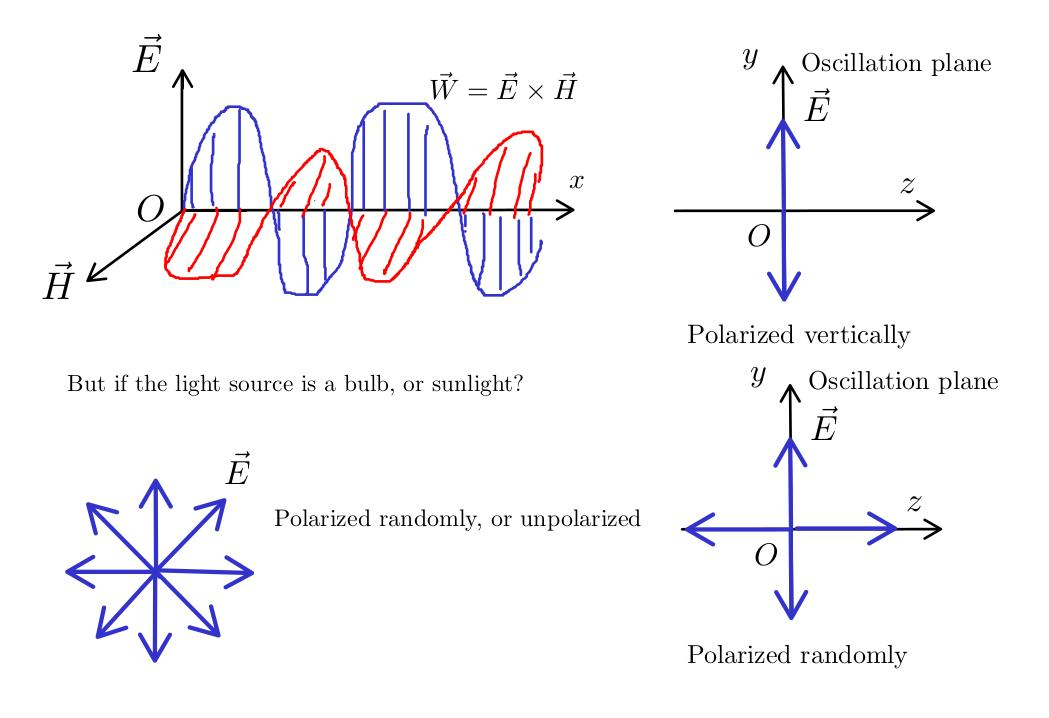
\includegraphics[width=0.9\textwidth]{polar.jpg}
			\caption{Polarization phenomenon}			\label{fig:re2}
\end{figure}

\end{frame}
\begin{frame}{Các tham số cơ bản của Antenna}
\begin{figure}[h]
			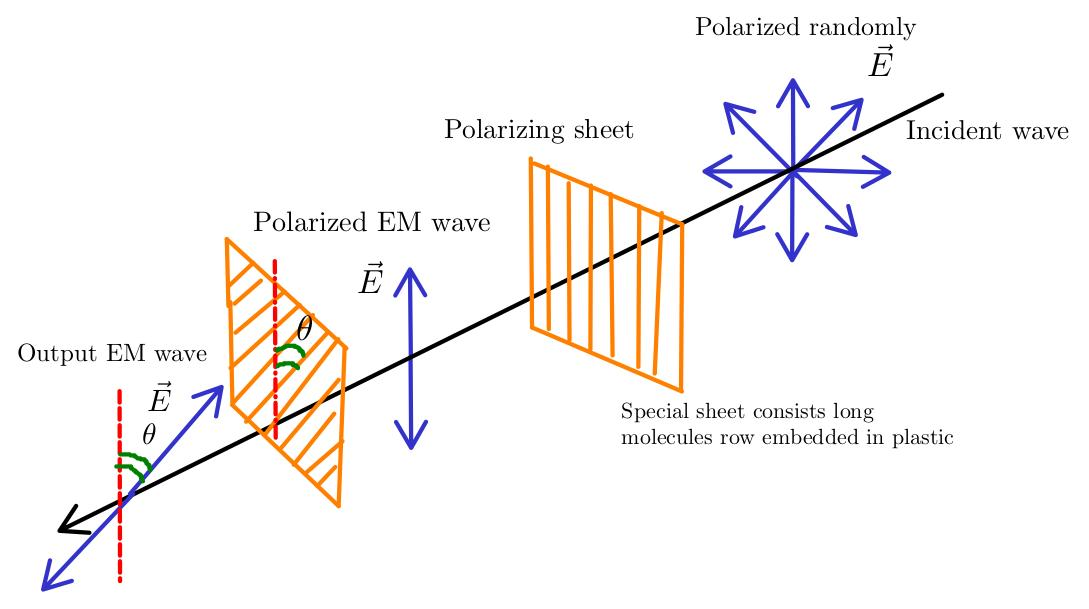
\includegraphics[width=0.7\textwidth]{incident.jpg}
			\caption{Pass EM wave through polarzating sheets}			\label{fig:re2}
\end{figure}
Giả sử sóng EM ban đầu có độ chiếu xạ là $W_{0}$:\\
Sau khi đi qua tấm phân cực 1: $$W_{1}=\frac{1}{2}W_{0}\;\text{(one-half rule)}$$
\\ Sau khi đi qua tấm phân cực 2: $$W_{2}=W_{1}\cos^2{\theta}\;\text{(cosine-squared rule)}$$
\end{frame}
\begin{frame}{Các tham số cơ bản của Antenna}
\subsection{Reflection coefficient}
\begin{itemize}
\item Reflection coefficient
\end{itemize}
Một hệ thống antenna bất kì có thể được mô hình hóa bằng mạch điện sau:
\begin{figure}[h]
			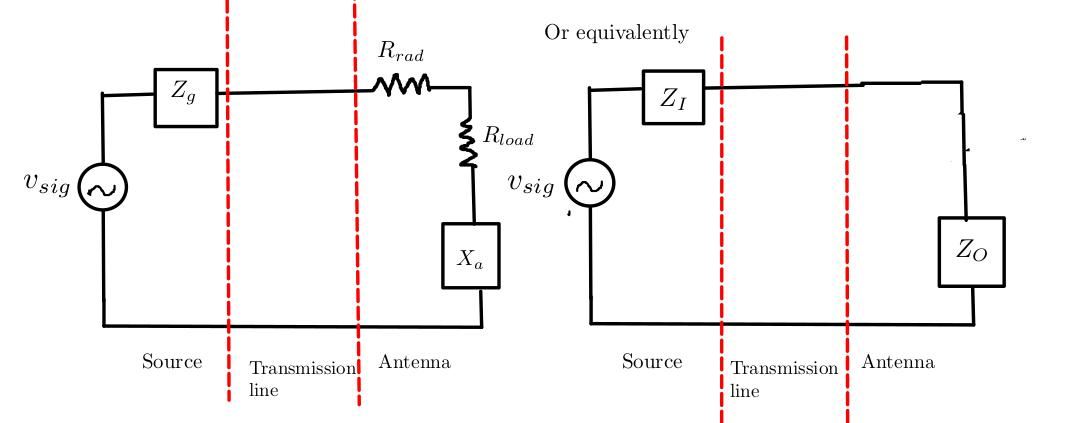
\includegraphics[width=0.7\textwidth]{circuit.jpg}
			\caption{Antenna equivalent circuit model}			\label{fig:re2}
\end{figure}
Trước khi đi sâu vào phân tích mô hình, ta hãy thử đặt một vấn đề tưởng chừng rất đơn giản, đó là sóng EM lan tỏa như thế nào trong mạch điện này ? Ngay từ những lập luận cơ sở từ slide lab 0, ta đã đều đồng ý với mô hình sóng EM chỉ lan tỏa ra ngoài môi trường từ antenna, phần mạch điện phía trước hoàn toàn không ảnh hưởng. Thế nhưng ở đây ta lại đang xét hệ số phản xạ (reflection coefficient) của sóng EM; tức giống như sóng cơ học, sóng EM phải bị "va chạm" hoặc chịu một thay đổi đột ngột nào đó (có thể như impedance chẳng hạn) thì mới có thể tạo ra sóng phản xạ. 
\\$\Rightarrow$ Mô hình ban đầu có vẻ như không thể giải thích hợp lý hiện tượng sóng EM phản xạ vì rõ ràng, sóng EM không hề chịu thay đổi đột ngột nào để phản xạ lại, nên việc định nghĩa hệ số phản xạ là vô nghĩa.
\end{frame}
\begin{frame}{Các tham số cơ bản của Antenna}
Ở đây, ta sẽ thử phân tích định tính mô hình đã được đưa ra thảo luận rất nhiều trên kênh YouTube Veritasium giải thích cách sóng EM được truyền đi trong mạch điện (mặc dù gây tranh cãi nhưng thật sự rất có cơ sở logic và đã được kiểm chứng bằng tính toán): 
\begin{figure}[h]
			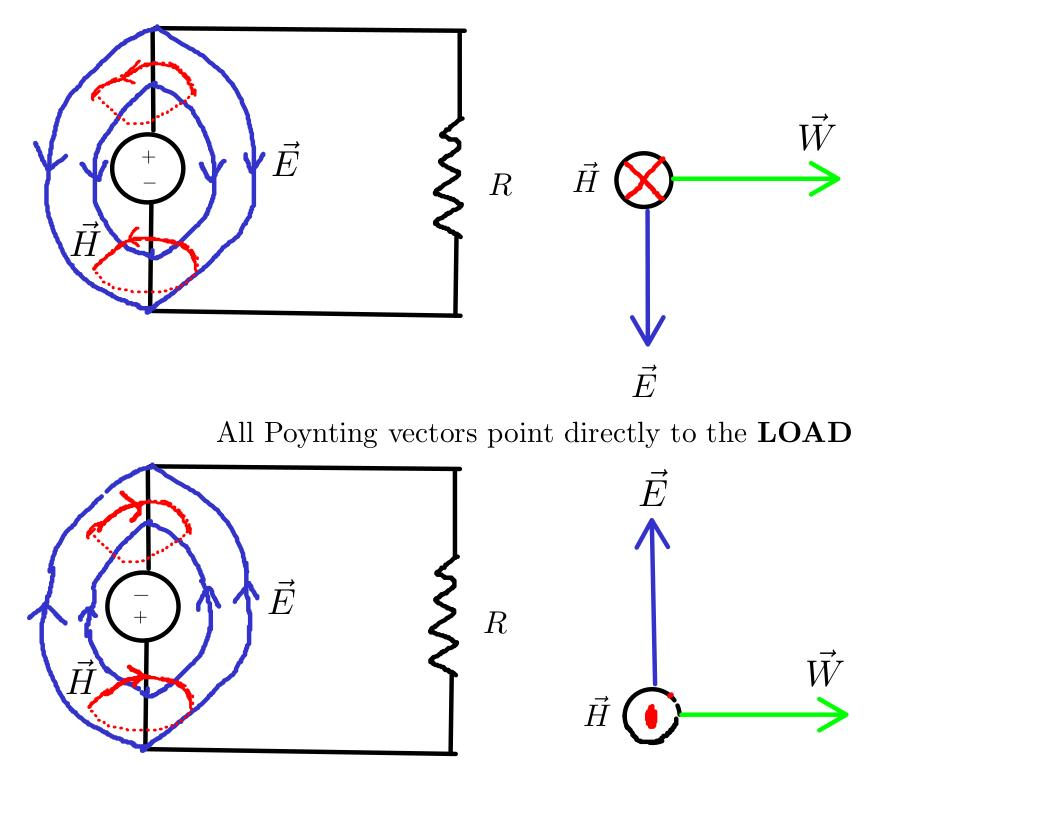
\includegraphics[width=0.7\textwidth]{poynting.jpg}
			\caption{Using Poynting vector model to explain how EM wave flows}			\label{fig:re2}
		\end{figure}
\end{frame}
\begin{frame}{Các tham số cơ bản của Antenna}
	Theo như mô hình vật lý trên, sóng EM hay năng lượng từ nguồn lan tỏa ngoài không gian chứ \textbf{không phải trong dây dẫn} cho đến tải (hay trở kháng phức), và điều này chứng tỏ sóng EM trước khi ra đến antenna có va chạm (thay đổi trở kháng đột ngột) với các linh kiện trong mạch điện để phản xạ một phần rồi sau đó mới lan tỏa. Với mô hình này, \alert{hệ số phản xạ có ý nghĩa}.
\\Trở lại vấn đề chính, sử dụng mô hình "Antenna equivalent circuit model", ta phân tích cách tính tham số $\Gamma$ (hệ số phản xạ):
\\ Xét một sóng EM được tạo ra và lan truyền theo mô hình đã trình bày ở trên, sóng khi gặp trở kháng ra $Z_{O}$ đã bị phản xạ một phần, ta giả sử hướng sóng EM truyền đi theo chiều dương trục $Ox$, và các kí hiệu tương ứng $+$, $-$ biểu thị sóng truyền đi và phản xạ lại.
\\ Từ định luật Ohm, ta có:
$$Z_{I}=\frac{V_{I}^+}{I_{I}^+}=-\frac{V^-_{I}}{I^-_{I}}\quad Z_{O}=\frac{V^+_{O}}{I^+_{O}}=-\frac{V^-_{O}}{I^-_{O}}$$
Với $\beta=\frac{2\pi}{\lambda}$ là hệ số sóng (wave number) của sóng EM, đại lượng đặc trưng cho sự biến đổi về pha theo không gian, ta viết lại biểu thức hàm $V^+$ và $V^-$ (bỏ qua yếu tố biến đổi pha về mặt thời gian do tần số của chúng như nhau):
$$V_{O}=V_{I}^+ e^{j\beta x}+V_{I}^- e^{-j\beta x}$$
$$I_{O}=I_{I}^+ e^{j\beta x}+I_{I}^- e^{-j\beta x}$$
$$\Rightarrow Z_{O}=\frac{V_{I}^+ e^{j\beta x}+V_{I}^- e^{-j\beta x}}{I_{I}^+ e^{j\beta x}+I_{I}^- e^{-j\beta x}}$$
\end{frame}
\begin{frame}{Các tham số cơ bản của Antenna}
Nếu xét gốc tọa độ tại $Z_{L} (???)$ và biến đổi tương đương (khá tricky), ta thu được:
$$\Gamma=\frac{V_{I}^-}{V_{I}^+}=\frac{Z_{O}-Z_{I}}{Z_{O}+Z_{I}}$$
và ta gọi $\Gamma$ là \alert{hệ số phản xạ}.
\\Ta tiếp tục định nghĩa SWR (Standing wave ratio) và RL (Return loss):
$$SWR=\frac{1+|\Gamma|}{1-|\Gamma|}$$
$$RL=-20\log_{10}|\Gamma|$$
Hiển nhiên, để tối ưu độ hiệu quả truyền sóng EM thì $\Gamma=0$, tương ứng với $SWR=1$ và $RL=+\infty$. Ta suy ra được một kết quả cực kì quan trọng (sẽ được chứng minh bằng một cách khác ở phần sau), đó là:
$$\Gamma=0\Leftrightarrow Z_{I}=Z_{O}$$
\end{frame}
\begin{frame}{Các tham số cơ bản của Antenna}
\subsection{Antenna Efficiency}
\begin{itemize}
	\item Antenna Efficiency
\end{itemize}
Từ mô hình mạch tương đương của Antenna, ta có thể nhận thấy rằng sự hao hụt trong quá trình truyền sóng chủ yếu gây ra do sự mất mát năng lượng dạng nhiệt tỏa ra trên điện trở, và hiện tượng sóng phản xạ tại trở kháng gây ra các điểm "dừng" (standing):
$$e_{0}=e_{r}e_{c}e_{d}=(1-|\Gamma|^2)e_{c}e_{d}$$
với: $e_{0}$ là hiệu suất tổng (total efficiency), $e_{r}$ là hiệu suất mismatch impedance, $e_{c}$ và $e_{d}$ là hiệu suất dẫn truyền và điện môi (tạm thời ta bỏ qua do 2 hệ số này rất khó để tìm và chỉ có thể thu được từ thực nghiệm). Hiển nhiên, nếu $\Gamma=1$ thì $Z_{I}=0$ và $e_{0}=0$
\subsection{Gain and Realized Gain}
\begin{itemize}
	\item Relative gain and realized gain
\end{itemize}
Độ lợi (gain) của antenna được định nghĩa là tỉ lệ giữa cường độ bức xạ tại \text{một hướng cho trước} với cường độ bức xạ đẳng hướng. Dễ thấy, khác với $D(\phi,\theta)$ là một hàm số, $G$ là hằng số với mỗi cặp biến góc cho trước.
\\ Ta định nghĩa hai khái niệm gain:
\begin{enumerate}
	\item Relative gain: $$G=\frac{4\pi U(\phi,\theta)}{P_{in}}$$
	\item Realized gain: $$G_{re}=e_{0} G=e_{0}\frac{4\pi U(\phi,\theta)}{P_{in}}$$
\end{enumerate}
\end{frame}
\begin{frame}{Các tham số cơ bản của Antenna}
Ví dụ: một onmidirectional antenna có hàm: $$U(\phi,\theta)=B_{0}\sin^3{\theta}$$
Hãy xác định giá trị cực đại của $G_{re}$ biết $Z_{I}=73\Omega$ và $Z_{O}=50\Omega$.
\\  Ta có:
\begin{equation*}
\begin{split}
	\textbf{max }G_{re}=e_{0}\frac{4\pi U(\phi,\theta)}{P_{in}}=(1-|\Gamma|^2)\frac{4\pi B_{0}\sin^3{\theta}}{B_{0}\iint_{S}U(\phi,\theta)d\Omega}=1.6382
\end{split}
\end{equation*}
Đổi ra thang dB: $$\textbf{max }G_{re}=10log_{10}(1.6382)=2.2865dB$$
\begin{itemize}
	\item  Beam Efficiency
\end{itemize}
 Hiệu suất chùm được định nghĩa là tỷ số giữa năng lượng bức xạ tại một góc $\theta$ nào đó với năng lượng bức xạ đẳng hướng:
 $$BE=\frac{\iint_{S'}U(\phi,\theta)d\Omega}{\iint_{S}U(\phi,\theta)d\Omega}$$
 với $S'$ là mặt kín bị giới hạn bởi góc $\theta$ và các dứ kiện đề bài cho khác, $S$ là toàn bộ mặt phẳng Oxyz.
\end{frame}
\begin{frame}{Hướng nghiên cứu tiếp theo}
	\section{Hướng nghiên cứu tiếp theo}
Nghiên cứu paper: Analysis and Experiment on Multi-Antenna-to-Multi-Antenna RF Wireless Power Transfer
\end{frame}
\end{document}

